\documentclass[a4paper, 14pt]{extreport}

\usepackage[utf8]{inputenc}
\usepackage[T2A]{fontenc}
\usepackage[english, russian]{babel}
\usepackage{listings}
\usepackage{amsmath,amssymb,amsfonts,amsthm}
\usepackage[left = 30mm, right = 10mm, top = 15mm, bottom = 20mm]{geometry}
\usepackage[pdftex]{graphicx}
\usepackage{color}
\usepackage{cancel}
\usepackage[hidelinks]{hyperref}
\usepackage{float}
\usepackage{subcaption}
\usepackage{indentfirst}
\usepackage{titlesec}

\titleformat{\chapter}[block]
  {\filcenter}
  {\thechapter}
  {1em}
  {\MakeUppercase}{}

\titleformat{\section}[block]
  {}
  {\thesection}
  {1ex}{}{}

\begin{document}
\selectlanguage{russian}
\begin{titlepage}
	\begin{center}
		\textsc{Федеральное государственное автономное образовательное учреждение высшего образования\\[2mm] 
			<<Санкт-Петербургский политехнический университет Петра Великого>>\\[18mm]
			Институт прикладной математики и механики\\[10mm]
			Высшая школа прикладной математики и вычислительной физики}
		\vfill
		\textsc{ОТЧЕТ ПО ЛАБОРАТОРНОЙ РАБОТЕ\\[2mm]
            по дисциплине: <<Математическая статистика>>\\[2mm]
			по теме: <<Гистограммы и плотности распределения>>}
	\end{center}
	\vfill
	
	\begin{minipage}{0.6\textwidth}
    ВЫПОЛНИЛ\\
    Сусоров Максим Анатольевич, \\
    ст. гр. 3630102/80101
	\end{minipage}
	\\\\
	
	\begin{minipage}{0.6\textwidth}
    ПРОВЕРИЛ\\
    Баженов Александр Николаевич, \\
    к.ф.-м.н., доц. ВШПМиВФ
	\end{minipage}
	
	\vfill
	\begin{center}	
		Санкт-Петербург, 2021
	\end{center}
\end{titlepage}	

\newpage
\tableofcontents

\chapter{Постановка задачи}

Даны 5 распределений:
\begin{enumerate}
	\item Нормальное распределение $N(x, 0, 1)$
	\item Распределение Коши $C(x, 0, 1)$
	\item Распределение Лапласа $L(x, 0, \frac{1}{\sqrt{2}})$
	\item Распределение Пуассона $P(k, 10)$
	\item Равномерное распределение $U(x, -\sqrt{3}, \sqrt{3})$	
\end{enumerate}
Для них требуется сгенерировать выборки размером 10, 50, 1000 элементов и построить на одном рисунке гистограмму и график плотности распределения.

\chapter{Теория}

\section{Рассматриваемые распределения}

\begin{itemize}
    \item Нормальное распределение 
	\begin{equation} \label{eq:Normal}
		N(x, 0, 1)=\frac{1}{\sqrt{2\pi}}e^{-\frac{x^2}{2}}
	\end{equation}
	
	\item Распределение Коши
	\begin{equation} \label{eq:Cauchy}
		C(x, 0, 1)=\frac{1}{\pi(x^2+1)}
	\end{equation}
	
	\item Распределение Лапласа
	\begin{equation} \label{eq:Laplace}
		L(x, 0, \frac{1}{\sqrt{2}})=\frac{1}{\sqrt{2}}e^{-\sqrt{2}|x|}
	\end{equation}
	
	\item Распределение Пуассона
	\begin{equation} \label{eq:Poisson}
		P(k, 10)=\frac{10^k}{k!}e^{-10}
	\end{equation} 
	
	\item Равномерное распределение
	\begin{equation} \label{eq:Uniform}
		U(x, -\sqrt{3}, \sqrt{3}) =
		\begin{cases}
			\frac{1}{2\sqrt{3}} & |x| \leq \sqrt{3} \\
			0 & |x|>\sqrt{3}
		\end{cases}
	\end{equation}	
\end{itemize}

\section{Гистограмма}

Гистограмма в математической статистике — это функция, приближающая плотность вероятности некоторого распределения, построенная на основе выборки из него \cite{Histogram}

\section{Построение гистограмм}

Графически гистограмма строится следующим образом. Сначала множество значений, которое может принимать элемент выборки, разбивается на несколько интервалов. Чаще всего эти интервалы берут одинаковыми, но это не является строгим требованием. Эти интервалы откладываются на
горизонтальной оси, затем над каждым рисуется прямоугольник. Если все интервалы были одинаковыми, то высота каждого прямоугольника пропорциональна числу элементов выборки, попадающих в соответствующий интервал. Если интервалы разные, то высота прямоугольника выбирается таким образом, чтобы его площадь была пропорциональна числу элементов выборки, которые попали в этот интервал \cite{Histogram}

\chapter{Результаты}

\section{Реализация}
\noindent
Исследование и построение гистограмм выполнено с помощью языка Python.
Исходный код выложен на GitHub, ссылка прикреплена в приложении \ref{code}

\section{Гистограммы и графики плотности распределения}

\begin{figure}
    \centering
    \begin{subfigure}[b]{0.5\textwidth}
    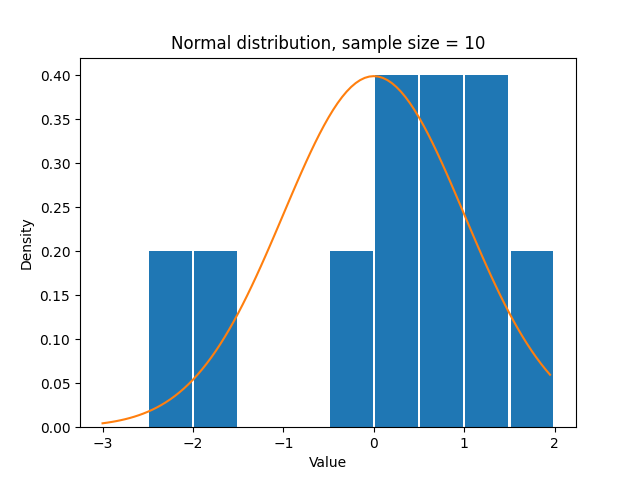
\includegraphics[scale = 0.5]{pics/Normal distribution_10.png}
    \caption{Размер выборки - 10}
    \end{subfigure}
    
    \begin{subfigure}[b]{0.5\textwidth}
    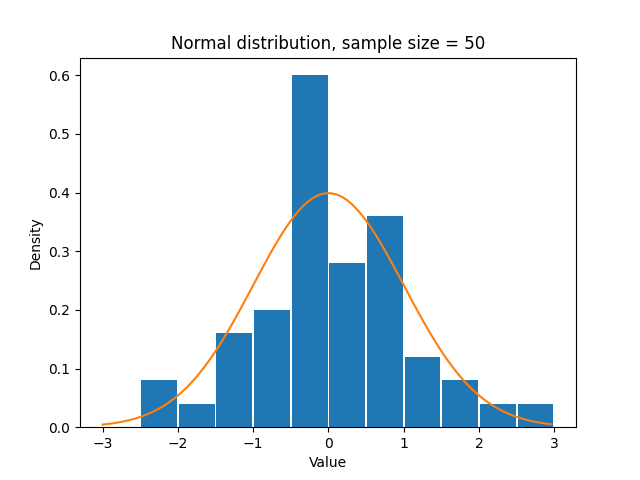
\includegraphics[scale = 0.5]{pics/Normal distribution_50.png}
    \caption{Размер выборки - 50}
    \end{subfigure}
    
    \begin{subfigure}[b]{0.5\textwidth}
    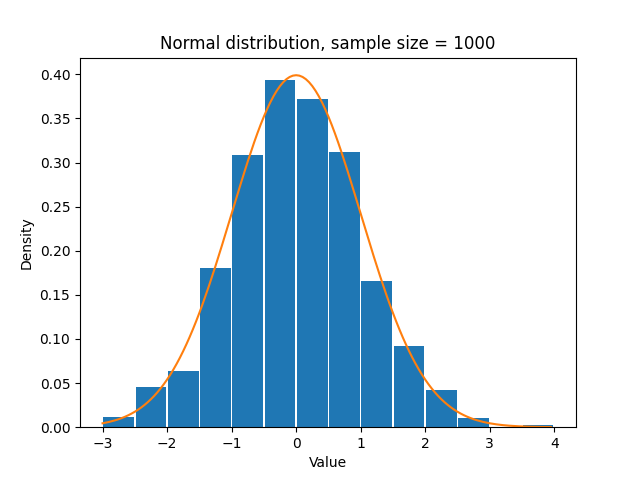
\includegraphics[scale = 0.5]{pics/Normal distribution_1000.png}
    \caption{Размер выборки - 1000}
    \end{subfigure}
    \caption{Нормальное распределение}
    \label{fig:normal}
\end{figure}

\begin{figure}
    \centering
    \begin{subfigure}[b]{0.5\textwidth}
    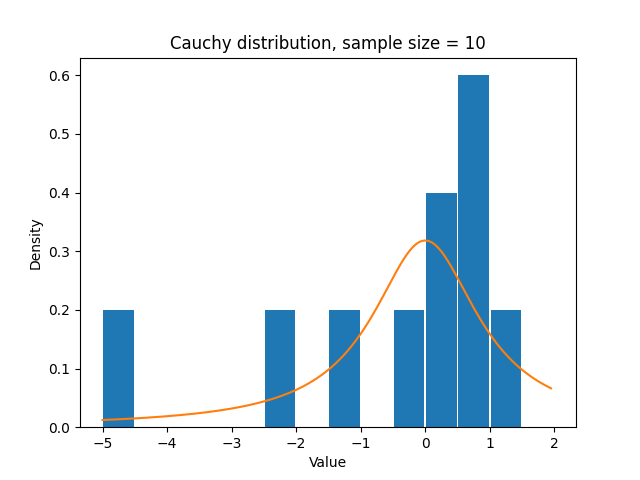
\includegraphics[scale = 0.5]{pics/Cauchy distribution_10.png}
    \caption{Размер выборки - 10}
    \end{subfigure}
    
    \begin{subfigure}[b]{0.5\textwidth}
    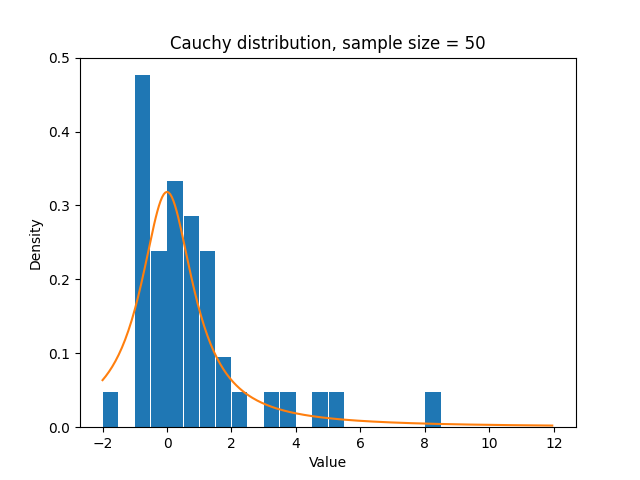
\includegraphics[scale = 0.5]{pics/Cauchy distribution_50.png}
    \caption{Размер выборки - 50}
    \end{subfigure}
    
    \begin{subfigure}[b]{0.5\textwidth}
    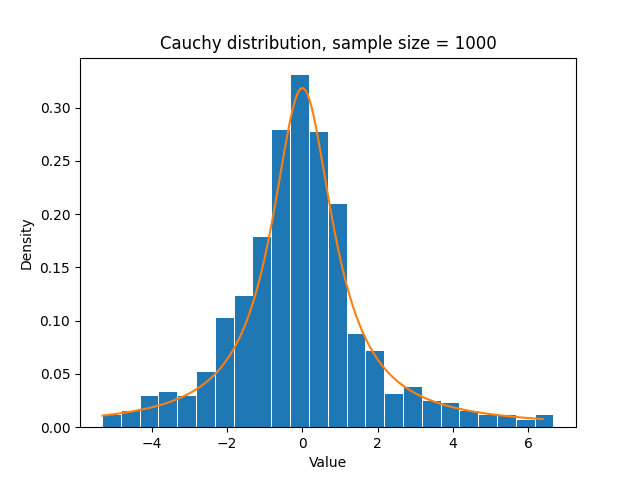
\includegraphics[scale = 0.5]{pics/Cauchy distribution_1000.png}
    \caption{Размер выборки - 1000}
    \end{subfigure}
    \caption{Распределение Коши}
    \label{fig:cauch}
\end{figure}

\begin{figure}
    \centering
    \begin{subfigure}[b]{0.5\textwidth}
    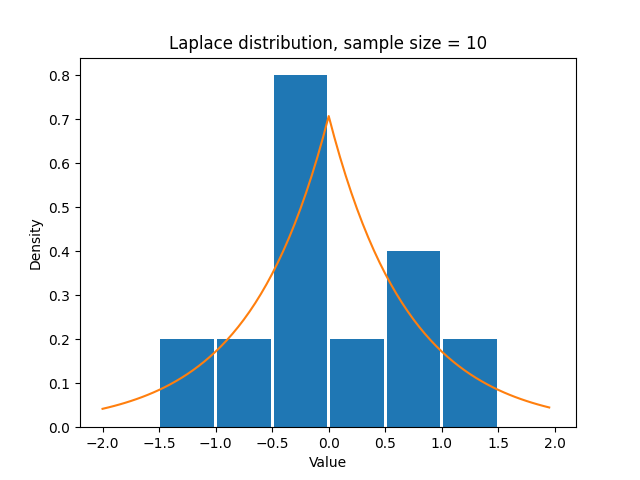
\includegraphics[scale = 0.5]{pics/Laplace distribution_10.png}
    \caption{Размер выборки - 10}
    \end{subfigure}
    
    \begin{subfigure}[b]{0.5\textwidth}
    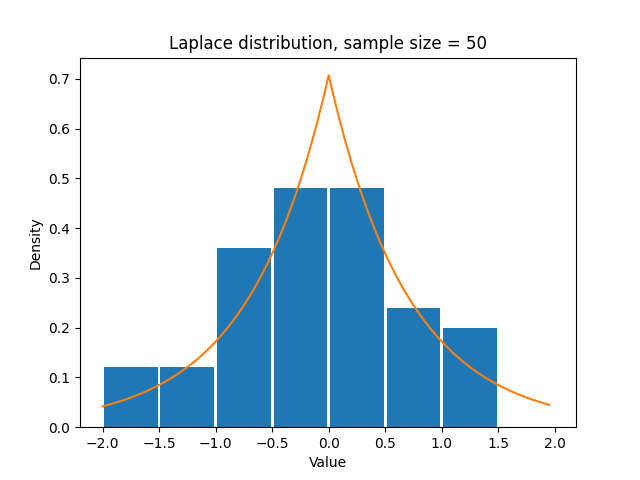
\includegraphics[scale = 0.5]{pics/Laplace distribution_50.png}
    \caption{Размер выборки - 50}
    \end{subfigure}
    
    \begin{subfigure}[b]{0.5\textwidth}
    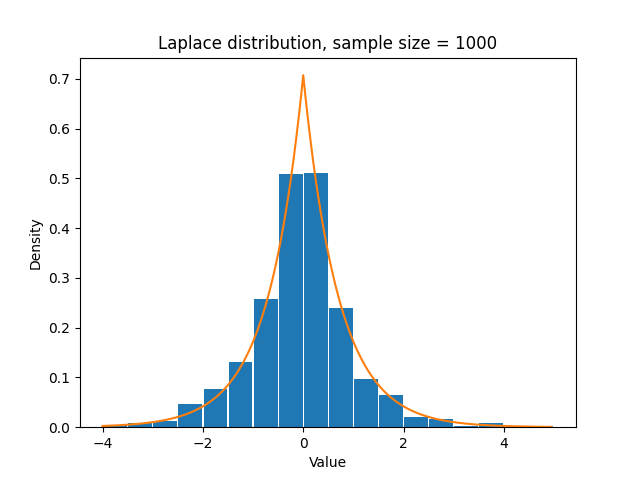
\includegraphics[scale = 0.5]{pics/Laplace distribution_1000.png}
    \caption{Размер выборки - 1000}
    \end{subfigure}
    \caption{Распределение Лапласа}
    \label{fig:laplace}
\end{figure}

\begin{figure}
    \centering
    \begin{subfigure}[b]{0.5\textwidth}
    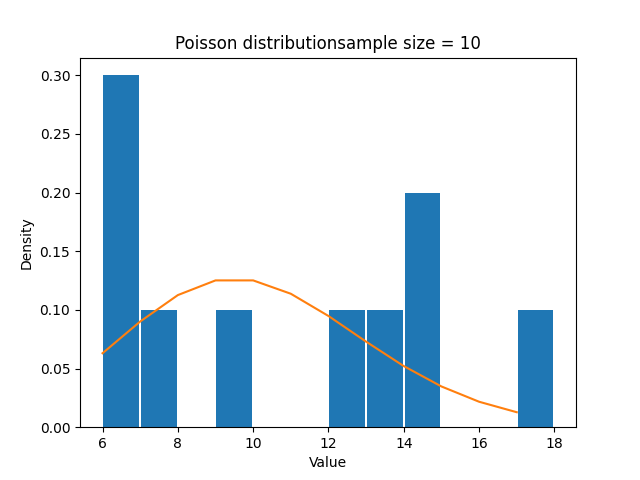
\includegraphics[scale = 0.5]{pics/Poisson distribution_10.png}
    \caption{Размер выборки - 10}
    \end{subfigure}
    
    \begin{subfigure}[b]{0.5\textwidth}
    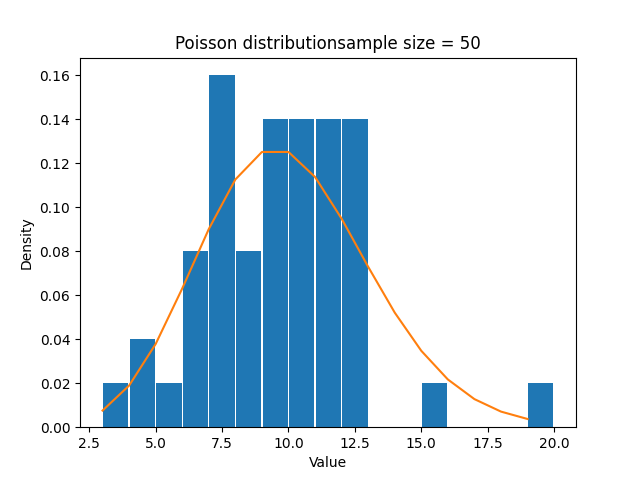
\includegraphics[scale = 0.5]{pics/Poisson distribution_50.png}
    \caption{Размер выборки - 50}
    \end{subfigure}
    
    \begin{subfigure}[b]{0.5\textwidth}
    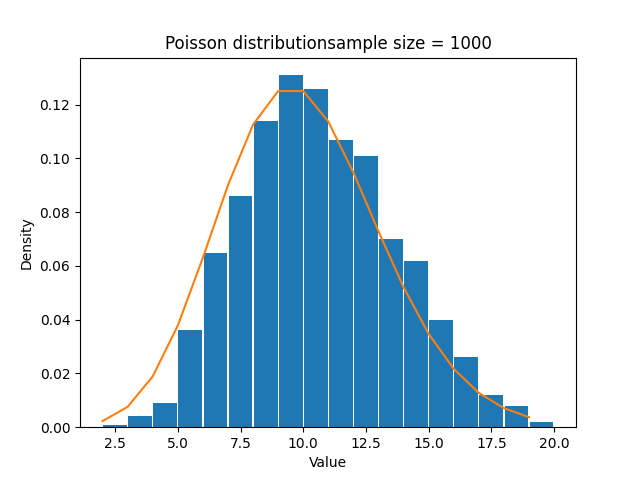
\includegraphics[scale = 0.5]{pics/Poisson distribution_1000.png}
    \caption{Размер выборки - 1000}
    \end{subfigure}
    \caption{Распределение Пуассона}
    \label{fig:poisson}
\end{figure}

\begin{figure}
    \centering
    \begin{subfigure}[b]{0.5\textwidth}
    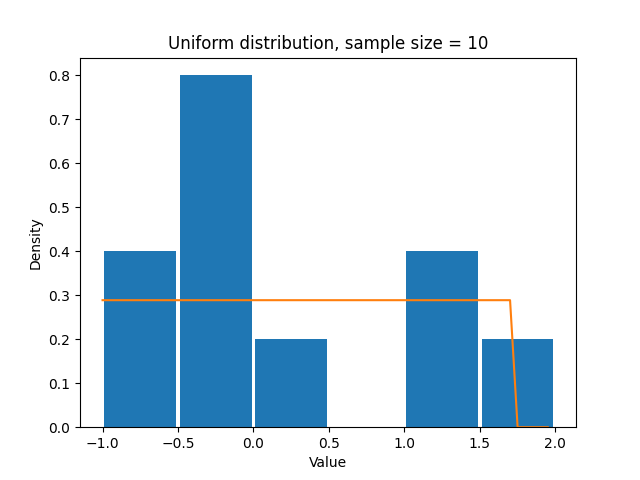
\includegraphics[scale = 0.5]{pics/Uniform distribution_10.png}
    \caption{Размер выборки - 10}
    \end{subfigure}
    
    \begin{subfigure}[b]{0.5\textwidth}
    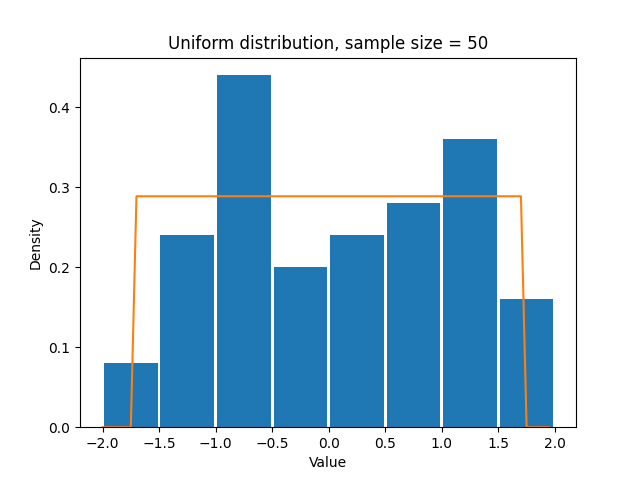
\includegraphics[scale = 0.5]{pics/Uniform distribution_50.png}
    \caption{Размер выборки - 50}
    \end{subfigure}
    
    \begin{subfigure}[b]{0.5\textwidth}
    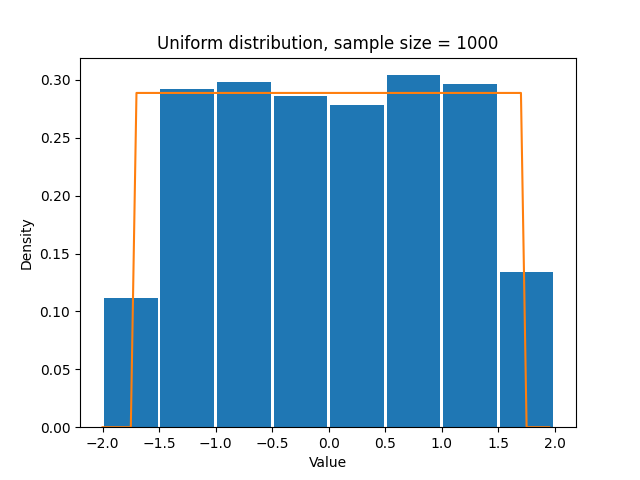
\includegraphics[scale = 0.5]{pics/Uniform distribution_1000.png}
    \caption{Размер выборки - 1000}
    \end{subfigure}
    \caption{Равномерное распределение}
    \label{fig:uniform}
\end{figure}

\chapter{Обсуждение результатов}

По гистограммам можем сделать следующий вывод --- чем больше размер выборки, тем лучше гистограмма, построенная по этой выборке, приближает функцию плотности вероятности.

Для выборки в 1000 элементов гистограммы нормального распределения, распределений Коши и Лапласа лучше всего приблизили графики их плотностей распределений.

Кроме того, на выборках малого размера хорошо заметны <<всплески>>.

\chapter{Приложение}

\noindent 1. Код работы: {\url{https://github.com/proted/SPbPU_MathStat}  \label{code}}

\begin{thebibliography}{1} 
    \addcontentsline{toc}{chapter}{\bibname}
	\bibitem{Histogram} Histogram. URL: {\url{https://en.wikipedia.org/wiki/Histogram}}
\end{thebibliography}

\end{document}
